\section{Definitions and notation}\label{sec:def}
In this report we consider a finite set of variables $\xx$ plus the set $\ie$ consisting of all inequalities and equalities over any subset of $\xx$. An element $c\in\ie$ is thus an equality or inequality over a subset $\VAR(c)\subseteq\xx$ and is referred to as an (in)equality over $\VAR(c)$. 
%\marginpar{argh, by my definition I cannot have two of the ``same'' inequality in an (in)equality system - maybe make it multisets?}
It can be written as
\begin{equation}\label{eq:ineq}
c: \sum_{x\in \VAR(c)}\coef(x,c)\cdot x\odot_c \rhs(c),
\end{equation} 
where $\odot_c\in\{=, \leq\}$ is the \emph{relation} of $c$, $\coef(x,c)\in\mathbb{R}$ is the \emph{coefficient} of $x$ in $c$ for any $x\in \VAR(c)$, and $\rhs(c)\in\mathbb{R}$ is the \emph{right-hand-side} of $c$.
%
Letting $\coef(x,c)= 0$ for all $x\in \xx\setminus\VAR(c)$, we can extend $c$ to $X$ for any set $X\subseteq \xx$ by letting $c_X$ be the (in)equality over $X$ given by
\begin{equation}\label{eq:constraintX}
c_{X}: \sum_{x\in X} \coef(x,c)\cdot x \odot_c\rhs(c).
\end{equation}
Assuming a given total order $\preceq$ on the variables in $\xx$ we can order and name the variable of any subset $X\subseteq \xx$ according to this order such that $X = \{x_1, x_2, \ldots, x_{|X|}\}$ and $x_1\prec x_2\prec \ldots \prec x_{|X|}$. 
Letting $\vea(c_X) \odef (\coef(x_1,c),\ldots,$ $\coef(x_{|X|},c))$ and $\ve{x}_X = (x_1,\ldots, x_{|X|})$, the constraint $c_X$ can also be written using the dot-product as $c_X:\vea(c_X)\cdot\ve{x}_X\odot_c \rhs(c)$. 
By definition $c_{\VAR(c)}$ equals $c$, so we let $\vea(c)\odef \vea(c_{\VAR(c)})$, and for convenience we leave out the subscript of $\ve{x}_X$ when the $X$ is implied e.g. by the coefficient vector in the dot product. 

We let $\var(c)$ denote the variables whose coefficient in $c$ is nonzero, i.e. $\var(c)\odef \set{x\in \VAR(c)}{\coef(x,c) \neq 0}$ $\subseteq \VAR(c)$, and we notice that we might have that $\var(c)\subset \VAR(c)$. When $VAR(c)$ is clear from context we allow ourselves to write $c$ as $c : \sum_{x\in \var(c)}\coef(x,c)\cdot x \odot_c \rhs(c)$.

The set of points in $\mathbb{R}^{|\VAR(c)|}$ that satisfies the (in)equality $c$ is called the \emph{feasible region} for $c$ and is hence defined as
\[
\feas(c) \odef \set{\ve{r}\in\mathbb{R}^{|\VAR(c)|}}{\vea(c)\cdot\ve{r}\odot_c \rhs(c)}.
\] 
Since the feasible region of an (in)equality is just a set of points in a (multi-dimensional) Euclidian space, here the order of the variables, $\prec$, is important and needs to be explicitly or implicitly given or assumed.
\\\\
In the following, an (in)equality system is a set $S$ of (in)equalities over the same set of variables, $\VAR(S)$, i.e. $S\subset\ie$ and $\VAR(c)=\VAR(S)$ for all $c\in S$. Therefore, when we union, intersect or subtract two (in)equality systems $S_1, S_2\subset \ie$ to produce another (in)equality system $S'$, it is required that all (in)equalities in $S'$ are (in)equalities over the same set $X$. Hence we require that $\VAR(S_1) = \VAR(S_2)$ when we talk about the (in)equality systems $S_1\cup S_2$, $S_1\cap S_2$ or $S_1\setminus S_2$. However, it is always possible to extend the (in)equalities in $S_1$ and $S_2$ to a common variable-set, and if $\VAR(S_1)\neq \VAR(S_2)$ we therefore let $S_1\cup S_2\odef \set{c_X}{c\in S_1}\cup \set{c_X}{c\in S_2}$, where $X=\VAR(S_1)\cup\VAR(S_2)$, and similar for the other set-operations $\cap$ and $\setminus$. 
%\marginpar{Alternatively, we could have that $S_1\sqcup S_2 \odef \set{c_{\VAR(S_1)\cup \VAR(S_2)}}{c\in S_1\cup S_2}$ etc.} \marginpar{Could have $\sqcup$ to make clear that its not just a set-operation on $\ie$} 

We let $\eqs(S)$ denote the set of equalities in $S$, i.e. $\eqs(S) \odef \set{c \in S}{\odot_c \text{ is } =}$, we define the used variables in $S$ as
$\var(S)\odef \cup_{c\in S}\var(c)$, and we let $S_X \odef \set{c_X}{c\in S}$ for any $X\subseteq \xx$.
The feasible region for $S$ is the set of points in $\mathbb{R}^{|\VAR(S)|}$ that satisfies \emph{all} (in)equalities in $S$, i.e. 
\[
\feas(S) \odef \cap_{c\in S}\feas(c).
\]
It follows that if $S_1, S_2\subseteq S$, then $\feas(S_1\cup S_2) = %\cap_{c\in S_1\cup S_2}\feas(c) = \cap_{c\in S_1}\feas(c)\cap\cap_{c\in S_2}\feas(c) = 
\feas(S_1)\cap \feas(S_2)$. 

In linear programming, it is common to have bounds for some of the variables in an (in)equality system $S$. For our purpose, upper and lower bounds are modeled as inequalities as in \eqref{eq:constraintX} with $X=\VAR(S)$ and a coefficient of $\pm 1$. If they exist, the inequalities representing upper and lower bounds for $x$ are referred to as $\UBc(x)$ and $\lbc(x)$, respectively, while $\UB(x)\in \mathbb{R}$ and $\lb(x)\in\mathbb{R}$ denote the upper, respectively lower bound of the variable $x$. 
That is, if the upper bound of $x$ exists, then $\UBc(x)$ refers to the inequality $x\leq \UB(x)$ in $S$, and if the lower bound of $x$ exists, then $\lbc(x)$ refers to the inequality $-x \leq -\lb(x)$ in $S$.

{We say that two (in)equality systems $S_1$ and $S_2$ are \emph{equivalent} and write $S_1\cong S_2$ if 
$\VAR(S_1)=\VAR(S_2)$ and $\feas(S_1) = \feas(S_2)$.}

An (in)equality $c\in S$ is \emph{redundant} if $c$ does not influence the feasible region for $S$, i.e. if $\feas(S)=\feas(S\setminus\{c\})$. The redundancy of an \emph{in}equality $c: \vea(c)\cdot\ve{x}\leq \rhs(c)$ can be determined by maximizing its left-hand-side:  
\begin{equation}\label{eq:redundant}
c \text{ is redundant iff }\max\set{\vea(c)\cdot\ve{r}}{\ve{r}\in \feas(S\setminus\{c\})} \leq \rhs(c).
\end{equation}
The equality $c: \vea(c)\cdot\ve{x} = \rhs(c)$ 
is redundant iff both inequalities 
$\vea(c)\cdot\ve{x} \leq \rhs(c)$ and $-\vea(c)\cdot\ve{x} \leq -\rhs(c)$ 
are redundant.
If the (in)equality $c$ is \emph{not} redundant, it is called \emph{non-redundant}.
%
\\\\
%\red{Is not needed, I guess: The feasible region of an (in)equality $c\in\ie$ defines one (if $c$ is an inequality) or two (if $c$ is an equality) halfspaces in $\mathbb{R}^{|\VAR(c)|}$, and therefore $\feas(S)$ is a polyhedron in $\mathbb{R}^{|\VAR(S)|}$.} 
%
As described, the feasible region of $S$ describes the combination of values for the variables in $\VAR(S)$ that satisfy all the (in)equalities in $S$. However, for the sake of abstraction there are some variables $Y\subseteq \VAR(S)$ whose value we are not interested in, we just want to know that a satisfying value for these variables exists.  
Therefore, we want to find a set of values $P$ for the variables of interest ($\VAR(S)\setminus Y$), such that when we have a set of values in $P$ then we can extend it with values for the variables in $Y$ in such a way that the collective set of values satisfy all (in)equalities in $S$. 
The {projection} of the feasible region of $S$ gives us the largest set of values with this property.

Let $S$ be an (in)equality system over $X$ and let $Y\subseteq X$ be the set of variables that we want to eliminate. Without loss of generality we can assume that $X = \{x_1,\ldots, x_{|X|}\}$, $x_1\prec \ldots \prec x_{|X|}$ and that $Y=\{x_i, x_{i+1}, \ldots, x_{|X|}\}$ for some $1\leq i\leq |X|$.
The {projection} of the polyhedron $\feas(S)$ with respect to $Y$ is then the polyhedron 
\[
\proj_Y\big(\feas(S)\big) \odef \set{\ve{r}\in\mathbb{R}^{|X\setminus Y|}}{\text{there exists an } \ve{r}'\in\mathbb{R}^{|Y|}\text{ such that }
(\ve{r},\ve{r'})\in \feas(S)}.
\]
See Figure~\ref{fig:proj}. Here $(\ve{r},\ve{r'})$ denotes the vector $(r_1,\ldots, r_{|X\setminus Y|}, r'_1,\ldots, r_{|Y|})$ where $\ve{r}=(r_1,\ldots, r_{|X\setminus Y|})$ and $\ve{r'}=(r'_1,\ldots, r_{|Y|})$.

For convenience of notation we let $\proj_{Y'}\big(\feas(S)\big) = \proj_{Y'\cap \VAR(S)}(\feas(S))$ for any $Y'\subseteq \xx$.

\begin{figure}
	\centering
		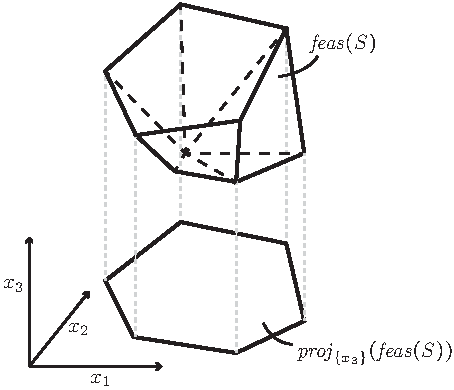
\includegraphics{figures/projection.pdf}
	\caption{Projection of the polyhedron $\feas(S)$ in $\mathbb{R}^3$ with respect to the third variable }
	\label{fig:proj}
\end{figure}
We notice that for arbitrary subsets $Y_1$ and $Y_2$ of $Y$ such that $Y_1\dot\cup Y_2=Y$,\footnote{$\dot\cup$ denotes disjoint union.} we have that $\proj_Y(P)=\proj_{Y_1}(\proj_{Y_2}(P))$. 
\\\\
In this report, we will only be interested in the projection of the feasible region of (in)equality systems,
and these are the feasible sets of (other) (in)equality systems (see e.g. \cite{ziegler95}). What we are interested in are the dependencies among the non-projected variables,  
so we want to talk about a system that ``generates'' a certain projection. For this we define $\prs_Y(S)$ to be the set of (in)equality systems whose feasible set is the projection of $S$ w.r.t. $Y$, i.e. 
\[
\prs_Y(S)\odef \set{S'\subset\ie}{\VAR(S')=\VAR(S)\setminus Y \text{ and }\feas(S') = \proj_Y\big(\feas(S)\big)}.
\]
If $S'\in\prs_Y(S)$ we say that $S'$ is a \emph{projection of $S$ w.r.t. $Y$}.
 
We point out, that for arbitrary (in)equality systems $S_1,S_2\subset \ie$ and $Y_1,Y_2\subseteq \xx$, the sets $\proj_{Y_1}(\feas(S_1))$ and $\proj_{Y_2}(\feas(S_2))$ are just sets of points in $\mathbb{R}^{|\VAR(S_1)\setminus Y|}$ and $\mathbb{R}^{|\VAR(S_2)\setminus Y|}$, respectively. As long as $|\VAR(S_1)|=|\VAR(S_2)|$ these sets can therefore be intersected, unioned or subtracted, but in order to have a meaningful interpretation of 
e.g. $\proj_{Y_1}(\feas(S_1))\cap\proj_{Y_2}(\feas(S_2))$ in our setting, we must have that $\VAR(S_1)\setminus Y_1 = \VAR(S_2)\setminus Y_2$, and projections must be given according to the same, implicitly given order $\prec$ on $\xx$.
%
\\\\
For proving the correctness of our decomposition in Section~\ref{sec:decomp} we need the following minor propositions.
\begin{restatable}{lemma}{projection}\label{lm:projection}
Let $S, S_1, S_2\subset\ie$ be (in)equality systems over $X$ and let $Y\subseteq X$. 
\begin{enumerate}
\item\label{lm:1.1} Assume that $\var(S_1)\cap\var(S_2) = \emptyset$. Then 
\begin{equation}\label{eq:lm1.1}
\proj_Y\big(\feas(S_1\cup S_2)\big) = \proj_Y\big(\feas(S_1)\big)\cap \proj_Y\big(\feas(S_2)\big).
\end{equation}
\item\label{lm:1.2} Assume that $\var(S_1)\cap Y = \emptyset$. Then
\begin{equation}
\proj_Y\big(\feas(S_1\cup S_2)\big) = \feas\big((S_1)_{X\setminus Y}\big)\cap \proj_Y\big(\feas(S_2)\big).
\end{equation}
\item\label{lm:1.3} Let $X'\subseteq \xx$ be a super set of $X$, i.e. $X\subseteq X'$, and let $E$ be an (in)equality system such that $\proj_Y\big(\feas(S)\big) = \feas(E)$.
Then 
\[
\proj_Y(\feas(S_{X'})) = \feas(E_{X'\setminus Y}).
\]
\end{enumerate}
\end{restatable}
\begin{proof} See Appendix.
\end{proof}
